\section{Intro to Deep Learning and Artificial Neural Networks}

\subsection{Introduction}\label{sec:ML_images}
As mentioned at the beginning of the chapter, deep learning is machine learning made with Deep Neural Networks.

Before starting to dive deeper into DNNs, let's talk for a second about digital images. It should be clear that a 2D Grayscale image is a 2D matrix, so it's a rank-2 tensor with shape (height, width). Instead, an RGB image is a 3D tensor with shape (height, width, channels), where $I(x, y) = [R(x, y), G(x, y), B(x, y)]$. There also exist 3D Grayscale images, which can be seen as a rank-3 tensor with shape (height, width, depth). They are vastly used in medicine, e.g. in computed tomography.

\begin{center}
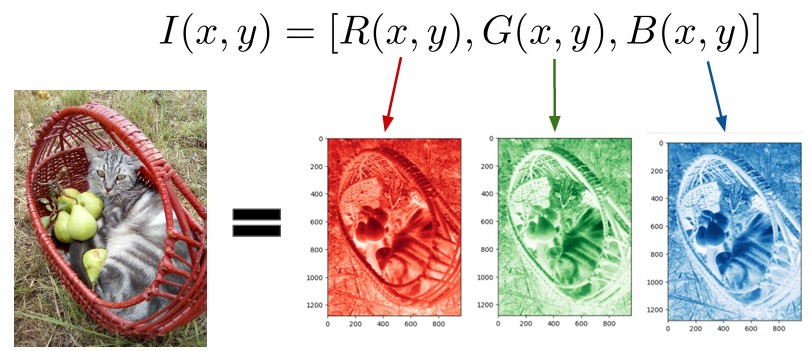
\includegraphics[width=0.6\textwidth]{figuresML/lesson_ml_1_pag_72.png} \\
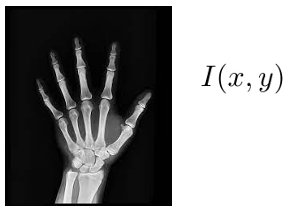
\includegraphics[width=0.25\textwidth]{figuresML/lesson_ml_1_pag_72a.png} \hspace{9mm}
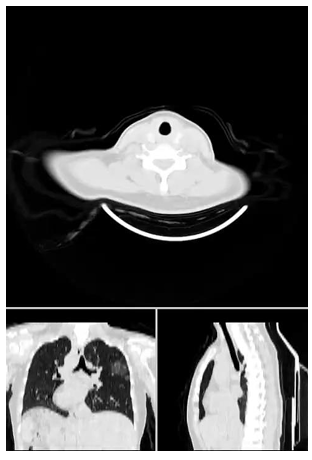
\includegraphics[width=0.25\textwidth]{figuresML/lesson_ml_1_pag_73.png}
\end{center}

\subsection{Logistic regression as a neural network}
Let's try to ease into DL starting from the concepts we are familiar with. Let's say for example that we want to write an algorithm which recognizes whether there is a cat in a given image. In our example (figure below), a $64 \times 64$ image can be flattened into an input vector with components $x_1$ to $x_n$. 
We can apply a linear transformation $wx + b$ followed by a sigmoid function $\sigma$, such that $\hat{y} = \sigma(\theta^T x) = \sigma(wx + b)$. Note that we have changed the notation just a little: the parameters are now called $w$ and not $\theta$ just because in DNNs we usually refer to them as \textbf{weights}.  

\begin{center}
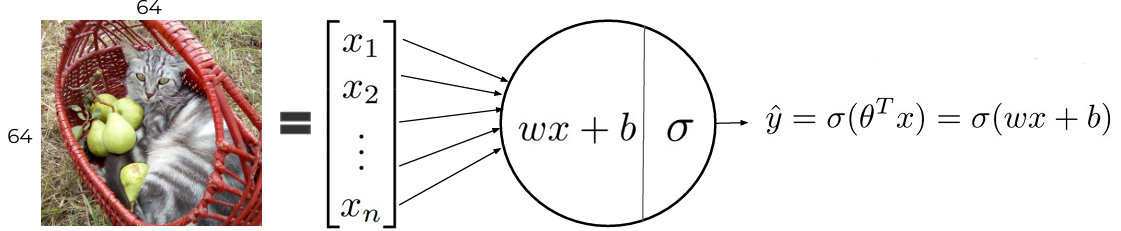
\includegraphics[width=0.85\textwidth]{figuresML/lesson_ml_1_pag_75.png}
\end{center}

We want to train this algorithm by following these steps:
\begin{enumerate}
    \item[-] Initialize weights and bias.
    \item[-] Find the optimal $w, b$.
    \item[-] Use them to predict $y$.
\end{enumerate}
In this case we could use a Binary Cross-Entropy as a loss function: 
\begin{equation}
    L(\theta) = -[y \log \hat{y} + (1-y)\log(1-\hat{y})]
\end{equation}
The output of this algorithm will be 1 if there is a cat, or 0 if there isn't: it should be clear that this is just a binary classification problem.

The circle representation in the figure above is what we call a \textbf{neuron}, and it is made of a \textbf{linear part} and an \textbf{activation function} (the sigmoid in our example). A \textbf{Deep Neural Network} can then be defined as a model composed of many neurons organized in \textbf{layers}.

Let's take another step forward by making our algorithm a little more complicated. Let's say that our goal now is finding a cat, a dog, or a bird in an image. To do so, we shall connect the input vector $x$ to multiple neurons, which we index using square brackets to indicate the layer as in the following figure. Of course, in doing so we are going to need three times the parameters used in the previous model. The activation functions for this first layer are:
\begin{itemize}
    \item[-] $\hat{y}_1 = a_1^{[1]} = \sigma(w_1^{[1]}x + b_1^{[1]})$
    \item[-] $\hat{y}_2 = a_2^{[1]} = \sigma(w_2^{[1]}x + b_2^{[1]})$
    \item[-] $\hat{y}_3 = a_3^{[1]} = \sigma(w_3^{[1]}x + b_3^{[1]})$
\end{itemize}
Each neuron will be responsible for a specific class (e.g., presence of a cat, dog, or bird) and in this case we must change the labels for the output:
\begin{itemize}
    \item[-] $[1, 0, 0]$ for the presence of a cat;
    \item[-] $[0, 1, 0]$ for the presence of a dog;
    \item[-] $[0, 0, 1]$ for the presence of a bird.
\end{itemize}
With this multi-class structure, we define the loss function as 
\begin{equation}\label{eq:4.17}
    L(\theta) = -\sum_{k=1}^{3}[y_k \log \hat{y}_k + (1-y_k)\log(1-\hat{y}_k)]
\end{equation} 
Notice that this is not yet a neural network since each output is totally independent of each other. 

\begin{center}
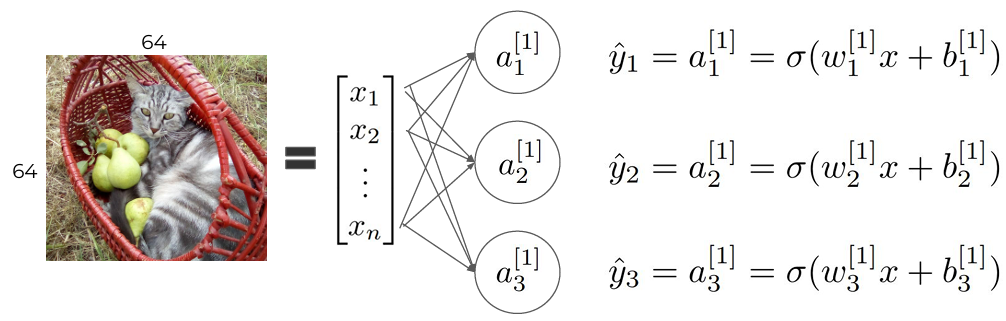
\includegraphics[width=0.85\textwidth]{figuresML/lesson_ml_1_pag_82.png}
\end{center}

Let's change one more time the problem by introducing the constraint that there is strictly a cat, a dog, or a bird. It will be useful to change our notation slightly, as shown in the figure below. We isolate the linear part and write it as such: $z_1^{[1]} = w_1^{[1]}x + b_1^{[1]}$. We also use the \textbf{softmax} function as our activation function:
\begin{equation}
a_1^{[1]} = \frac{e^{z_1^{[1]}}}{\sum_{k=1}^{3}e^{z_k^{[1]}}}
\end{equation}
The softmax introduces a relationship between the 3 neurons so that we obtain a (normalized) probability distribution between the classes instead of an independent probability for each class. For example, if in the image there is a cat with an 80\% probability, there could be a dog with 10\% probability and a bird with another 10\%. In this case, we should also change the output labels to a so-called \textit{one-hot encoding}: $[1, 0, 0]$, $[0, 1, 0]$, $[0, 0, 1]$ are the only possible labels (they do not combine as before). With softmax, we utilize the simpler cross-entropy loss function (since any predicted $y$ depends on all the other values, it is too hard to compute the derivative of Eq. \ref{eq:4.17}):
\begin{equation}
    L_{CE} = -\sum_{k=1}^{3} y_k \log(\hat{y}_k)
\end{equation}
Since there is a relationship between all the outputs, \textit{this is the first shallow example of a neural network}.

\begin{center}
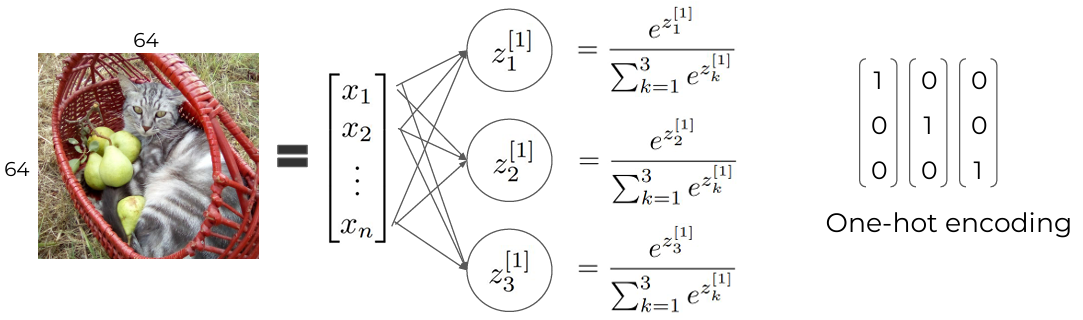
\includegraphics[width=0.85\textwidth]{figuresML/lesson_ml_1_pag_88.png}
\end{center}

\subsection{Neural Network architecture}
The following figure can be useful to understand the typical architecture of a neural network. First, the inputs $x$ are connected to the first layer of neurons called the \textbf{input layer}. Then all the neurons of the input layer are connected to all the neurons of the subsequent layer, creating a \textbf{fully connected layer}. The last layer is also called an \textbf{output layer} and all the layers which are not the input nor the output are called \textbf{hidden layers}. It should be clear now that a layer refers to neurons that are not connected to each other within the same depth level. When you build an architecture, the number of neurons in the output layer should match your problem, i.e., it should be equal to the number of classes: it usually defines the problem we would like to solve.

\begin{center}
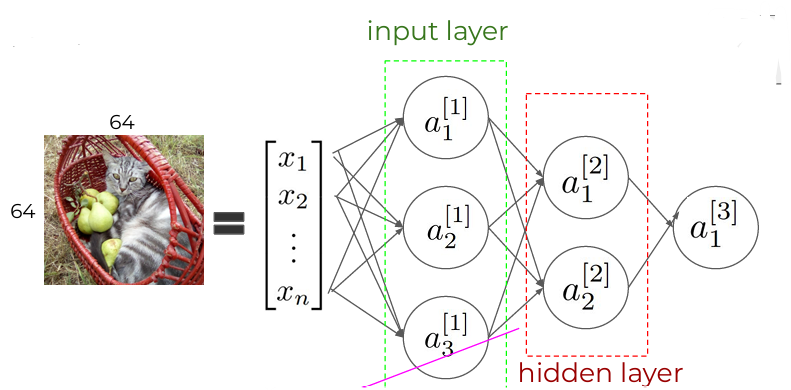
\includegraphics[width=0.75\textwidth]{figuresML/lesson_ml_1_pag_90.png}
\end{center}

Now, the learning scheme is quite the same as in the case of linear regression we have seen at the beginning of the chapter: at a certain point we will find a loss function and use the gradient descent method to minimize it. The difference is that before doing this, we need to pass through the entire structure of our neural network. The process works through \textbf{forward propagation}: we process the input data according to the operation of the neuron sequentially (i.e. the last activation will be a function of the last $z$, which is a function of the previous activation, and so on), as shown below. 

\begin{center}
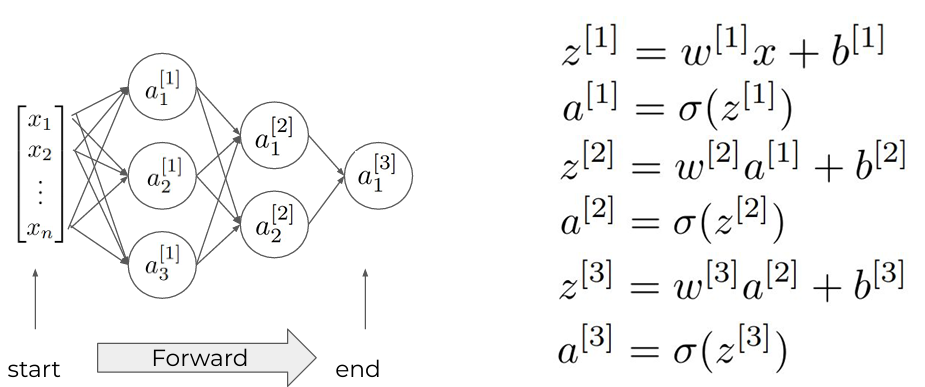
\includegraphics[width=0.75\textwidth]{figuresML/lesson_ml_1_pag_93.png}
\end{center}

Once we have computed the activation of the last layer, we have our prediction so we can compute the value of the loss function. To minimize this loss function using an optimization algorithm like Stochastic Gradient Descent, we need to \textbf{compute the derivatives of the loss function with respect to all the network weights}. 

As an example, let's try to do it explicitly for our neural network. Since it has only one neuron in the last layer, we are obviously trying to solve a binary classification task, so we will use the BCE as a loss function.

To clarify the notation:
\begin{itemize}
    \item[-] By \textit{cost function} we mean all the loss functions computed on a dataset ($m$ is the batch size): $J(\hat{y}, y) = \frac{1}{m}\sum_{i=1}^{m}L^{(i)}(\hat{y}, y)$.
    \item[-] By \textit{loss function} we mean the single error computation, e.g. BCE: \\ $L^{(i)} = -[y^{(i)}\log\hat{y}^{(i)} + (1-y^{(i)})\log(1-\hat{y}^{(i)})]$.
\end{itemize}
We compute the derivative of the loss with respect to $w^{[3]}$:
\begin{equation*}
    \frac{\partial L}{\partial w^{[3]}} = -\left[ y^{(i)} \frac{\partial}{\partial w^{[3]}} (\log(\sigma(w^{[3]}a^{[2]} + b^{[3]}))) + (1 - y^{(i)}) \frac{\partial}{\partial w^{[3]}} (\log(1 - \sigma(w^{[3]}a^{[2]} + b^{[3]}))) \right]
\end{equation*}
which, after a few simple mathematical steps becomes:
\begin{equation}
\frac{\partial L}{\partial w^{[3]}} = -(y^{(i)} - a^{[3]})a^{[2]}
\end{equation}
Using the chain rule, we can compute the derivative with respect to $w^{[2]}$:
\begin{equation*}
\frac{\partial L}{\partial w^{[2]}} = \frac{\partial L}{\partial a^{[3]}} \frac{\partial a^{[3]}}{\partial z^{[3]}} \frac{\partial z^{[3]}}{\partial a^{[2]}} \frac{\partial a^{[2]}}{\partial z^{[2]}} \frac{\partial z^{[2]}}{\partial w^{[2]}}
\end{equation*}
We know exactly how to compute each of those partial derivatives because we have
\begin{equation}
\begin{aligned}
z^{[1]} &= w^{[1]}x + b^{[1]} \quad \quad \ \  a^{[1]} = \sigma(z^{[1]}) \\
z^{[2]} &= w^{[2]}a^{[1]} + b^{[2]} \quad\quad a^{[2]} = \sigma(z^{[2]}) \\
z^{[3]} &= w^{[3]}a^{[2]} + b^{[3]} \quad\quad a^{[3]} = \sigma(z^{[3]})
\end{aligned}
\end{equation}
We also know that the derivative of the sigmoid is nicely defined as $g'(z) = g(z)(1-g(z))$, so 
\begin{equation*}
    \dfrac{\partial a^{[i]}}{\partial z^{[i]}} = a^{[i]}(1-a^{[i]})  
\end{equation*}
Lastly: 
\begin{equation*}
    \frac{\partial L}{\partial a^{[3]}} \frac{\partial a^{[3]}}{\partial z^{[3]}} = \dfrac{\partial L}{\partial z^{[3]}}=\dfrac{\partial L}{\partial w^{[3]}} / \dfrac{\partial z^{[3]}}{\partial w^{[3]}}
\end{equation*}
Putting everything together we get:
\begin{equation}
    \frac{\partial L}{\partial w^{[2]}} = w^{[3]} a^{[2]} (1 - a^{[2]}) (a^{[3]} - y^{(i)}) a^{[1]}
\end{equation}

The same thing can be done for $\dfrac{\partial L}{\partial w^{[1]}}$. This kind of derivative computation for the loss function is called \textbf{backpropagation} and it is extremely efficient because many terms of the derivatives are already computed in the forward pass (like $a^{[1]}$, $a^{[2]}$, $a^{[3]}$) or in the previous derivatives. Caching them makes backpropagation computationally convenient. 

With that said, we have a pretty good understanding of the training cycle of a neural network: 
\begin{enumerate}
    \item Forward pass of the data
    \item Computation of the loss function
    \item Computation of the derivatives of the loss function through backpropagation
    \item Minimization of the loss function and optimization of the weights (e.g through SGD)
    \item Repeat until convergence
\end{enumerate}
An entire pass of the training dataset through the learning algorithm (1-4) is called an \textbf{epoch}.
We can update the network in different ways during training:
\begin{enumerate}
    \item Update the weights for each training point (very time consuming).
    \item Update the weights for a mini-batch of data (less time consuming).
\end{enumerate}

\hrulefill

\subsubsection{Note: A very brief and incomplete history of NN}
Machine learning systems have been around for many years, but what has changed nowadays is the arrival of Deep Learning! The history of AI is characterized by periods of time often referred to as \textit{AI winters} where technology could not keep up with theory, as the computational power available was not enough for machine learning purposes.  Here are some meaningful milestones:
\begin{itemize}
    \item[-] 1957 - Rosenblatt introduces the \textit{perceptron} (see below).
    \item[-] 1962 - Rosenblatt used the term backpropagation which will become the mathematical algorithm for doing feedback in practice.
    \item[-] 1980 - Fukushima introduces the \textit{neocognitron}.
    \item[-] 1998 - LeCun published the first Neural Network that is able to work directly with images!
    \item[-] 2006 - Chellapilla proposed using GPUs to boost NN training.
    \item[-] 2006 - 2012 - Many technologies evolved, the amount of available data increased until 2012 when something very interesting happened (we will soon see).
\end{itemize}
\hrulefill

\subsection{Multi-Layer Perceptron and Deep Feed Forward Network}
The most common NN in the '90s was the \textbf{Multilayer Perceptron} (MLP). 
It features a graph structure organized in 3 layers (input, hidden and output), whose nodes are connected only from one layer to the next and all possible connections are present (fully connected), as shown below. There are no intra-layer connections and no direct connections from input to output. Size of input and output layers are fixed by the problem. Hyperparameters include the size of the hidden layers and the type of activation function, while the parameters to learn are the weights of the connections. It is nothing stranger than the simple example we have seen before.

\begin{center}
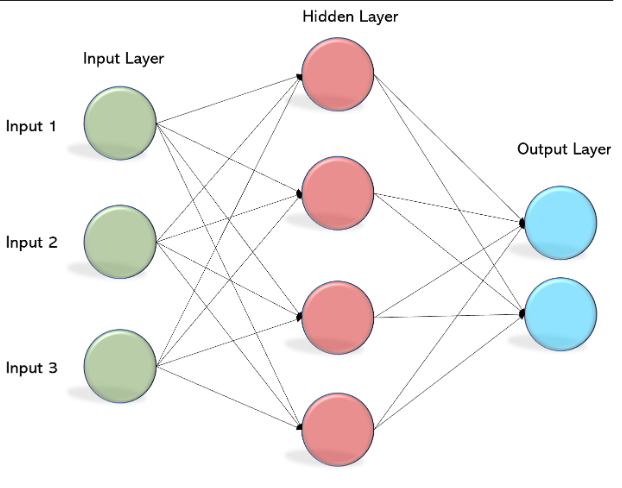
\includegraphics[width=0.4\textwidth]{figuresML/lesson_ml_1_pag_111.png}
\end{center}

The simplest extension to the MLP is to add more hidden layers (even hundreds or thousands), forming a \textbf{Deep Feed Forward Network} (or \textit{Deep Dense Network}). The hierarchical structure allows easier abstraction by the network, with early layers computing low-level features and deeper layers representing more abstract properties.

\begin{center}
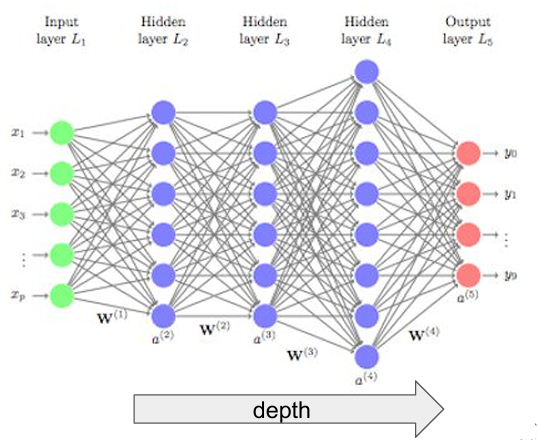
\includegraphics[width=0.65\textwidth]{figuresML/lesson_ml_1_pag_113.png}
\end{center}

\subsection{The importance of activation functions}
Let's now take a step back and ask ourselves: \textit{why do we need activation functions?} The "horse" problem shown below illustrates what happens if we do not use an activation function in a Neural Network i.e., if we do not introduce non-linearity. If we train a linear classifier on images of horses facing left or right, the learned weights look like a two-headed horse. There are no two-headed horses! \textbf{Non-linearity is required} (we will see why more thoroughly in Sec. \ref{sec:non_linearity}.

\begin{center}
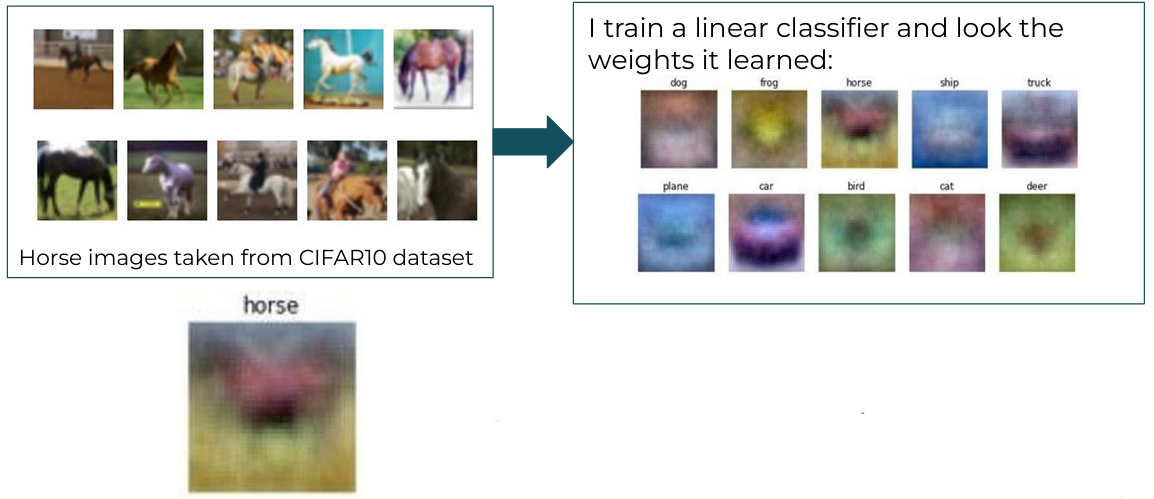
\includegraphics[width=0.9\textwidth]{figuresML/lesson_ml_1_pag_115.png}
\end{center}

There are many different activation functions:
\begin{itemize}
    \item[-] \textit{Linear}: $f(x) = x$. Of course it cannot be used in hidden layers (where non-linearity is mandatory) but it can be useful for output nodes in regression problems if the output values span a very wide range.
    \item[-] \textbf{Sigmoid}: $f(x) = \sigma(x) = \frac{1}{1+e^{-x}}$. It was used historically in hidden layers but leads to the \textit{vanishing gradient} problem. It can be useful in the last layer for binary classification problems with a single output or multi-label classifiers.
    \item[-] \textbf{Softmax}: $f_i(\vec{x}) = \frac{e^{x_i}}{\sum_{j=1}^{J}e^{x_j}}$. As seen, it is useful in classification problems with one-hot encoded multi-class labels.
    \item[-] \textbf{Rectified Linear Unit (ReLU)}: $f(x) = \max(0, x)$. It is usually the default for hidden layer activations (we will soon see why). Variants of ReLU include Leaky ReLU, Swish and Exponential Linear Unit (ELU).
    \item[-] \textit{tanh}: It is not widely used anymore, even though it was historically relevant.
    \item[-] \textit{Maxout}: $\max(w_1^T x + b_1, w_2^T x + b_2)$
\end{itemize}

\begin{center}
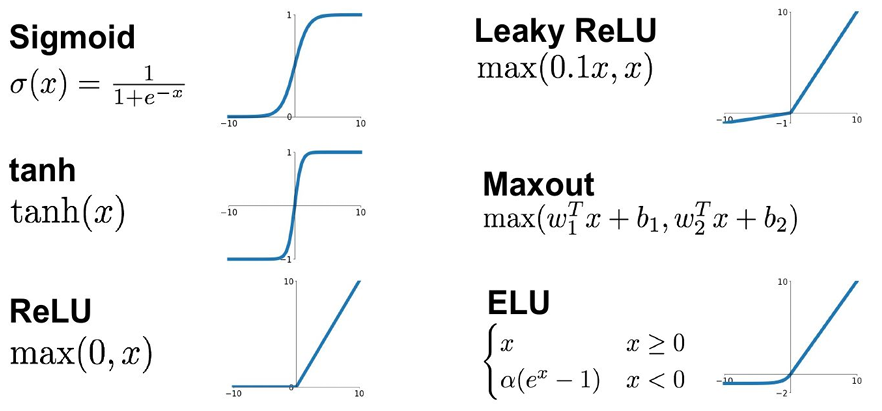
\includegraphics[width=0.65\textwidth]{figuresML/lesson_ml_1_pag_116.png}
\end{center}

It should be clear now that the choice of the activation function for the output layer is pivotal. Here we sum up the correct activation function, loss function, and output label for the three kinds of simple problems we have faced:
\begin{itemize}
    \item[-] \underline{Regression}: Since we want to have a continuous output, we use a linear activation. Loss: Mean Squared Error (MSE) or Mean Absolute Error (MAE). Label: continuous numbers.
    \item[-] \underline{Binary Classification}: We use a Sigmoid activation. Loss: Binary Cross-Entropy. Label: 0 or 1.
    \item[-] \underline{Multi-class Classification}: We use a Softmax activation. Loss: Categorical Cross-Entropy (or Sparse Categorical Cross-Entropy if labels are integers). Label: one-hot for CCE, integers for SCCE (0, 1, 2, 3, ...). Note that it is always better to use one-hot encoding for multi-class classification.
\end{itemize}

\subsection{A deeper look at overfitting and regularization}
As discussed previously, if the capacity is large enough the network could overfit on the training dataset. We must have a separate, statistically independent, validation/generalization sample to evaluate performance (with loss or other metrics). It should also be noticed that training results depend on many choices like the size of the data batches (usually limited by the memory of your GPU), learning rate (how much you move along the gradient at each iteration), chosen gradient descent algorithm, and capacity of the network. Take a look at the following figures to see what could really happen to your loss function during training (there is noise, a loss that dramatically increases at a certain point without a clear reason, and much more).

\begin{center}
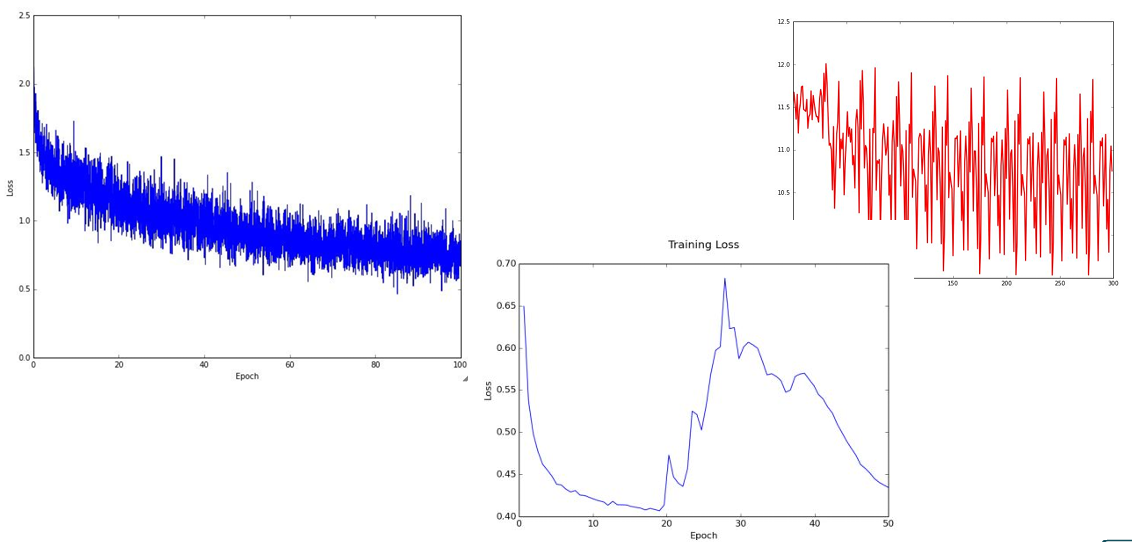
\includegraphics[width=0.65\textwidth]{figuresML/lesson_ml_1_pag_124.png}
\end{center}

Previously, we saw that adding a penalty to the loss function can induce regularization. 
A technique particularly suited for Fully Connected Neural Networks is called \textbf{dropout}: during training a fraction of nodes is discarded randomly at each iteration in order to "confuse" our algorithm. This makes the NN more robust to noise and effectively augments the input dataset, as shown below.

\begin{center}
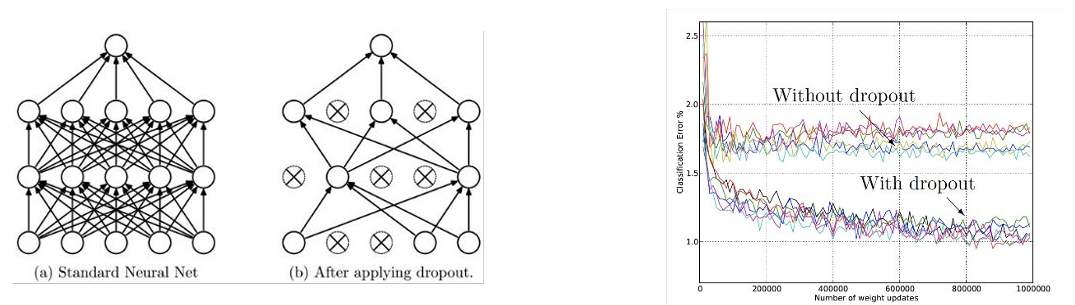
\includegraphics[width=0.95\textwidth]{figuresML/lesson_ml_1_pag_125.png}
\end{center}

As previously mentioned, weight updates can be performed for individual training points or across mini-batches of data. In the context of mini-batch training, \textbf{Batch Normalization (BN)} is a crucial technique designed to normalize the inputs of each hidden layer, ensuring they maintain a stable distribution throughout the training process. 

Specifically, BN calculates the mean and variance for the current mini-batch and uses them to center and scale the layer's activations. 

By keeping the input distribution relatively constant (mitigating a phenomenon known as \textit{internal covariate shift}) each layer does not have to continuously adapt to the changing weights of previous layers. This stability significantly speeds up convergence, allows for the use of much higher learning rates without the risk of divergence, and acts as a mild form of regularization (often reducing the need for techniques like dropout), ultimately leading to improved model generalization.

Proper scaling of input data is a mandatory preprocessing step when training neural networks. Unlike algorithms such as decision trees, where unscaled data merely shifts the split thresholds, neural networks are highly sensitive to input magnitudes. In other words, if the input values $z$ are too large or too small, they can cause activation functions (such as ReLU) to produce extreme outputs. This leads to \textit{network saturation}, a state where neurons lose their sensitivity to the data and effectively "die". If this saturation is allowed to propagate through the network's hidden layers, the model becomes completely untrainable. 

To prevent this and ensure all features operate within the same range, \textbf{input normalization or scaling} is strictly required. The most common approach is \textit{standardization}, which consists of centering the data by subtracting the mean and scaling it by dividing by the standard deviation.

\subsection{Introduction to Keras}
\textbf{Keras} is a Python library that allows you to build, train, and evaluate NNs. Nowadays the most used library is \texttt{torch} because GPT, Transformers and more complex architectures are written with it, and because it seems to be more efficient than \texttt{TensorFlow} (which Keras is a part of). However, in this kind of problem it is very hard to measure the actual efficiency (we will see why). 

Two different syntax methods are usable in Keras to build the network architecture:
\begin{itemize}
    \item[-] \textbf{Sequential}: simple "stack" of layers.
    \item[-] \textbf{Model (functional API)}: create more complex topologies.
\end{itemize}
Multiple types of layers are supported: \textit{dense} (classic fully connected layer), \textit{convolutional}, \textit{recurrent} and so on (we will see those too). It also provides multiple types of activation functions, various optimizers, and gradient descent techniques. Right now most programmers are using \textit{Adam}, which is a particular type of gradient descent algorithm (yes, this too will be a future topic of discussion). 

Below you can find some simple examples to start becoming familiar with this new module.

\subsubsection{- Keras first sequential example}

Here is how you can define a simple sequential model:

\begin{Verbatim}[label=\makebox{\url{https://github.com/lucabaldini/cmepda/tree/master/slides/latex/snippets/pima_classifier.py}},commandchars=\\\{\}]
\PY{c+c1}{\PYZsh{} Necessary modules}
\PY{k+kn}{from}\PY{+w}{ }\PY{n+nn}{numpy}\PY{+w}{ }\PY{k+kn}{import} \PY{n}{loadtxt}
\PY{k+kn}{from}\PY{+w}{ }\PY{n+nn}{keras}\PY{n+nn}{.}\PY{n+nn}{models}\PY{+w}{ }\PY{k+kn}{import} \PY{n}{Sequential}
\PY{k+kn}{from}\PY{+w}{ }\PY{n+nn}{keras}\PY{n+nn}{.}\PY{n+nn}{layers}\PY{+w}{ }\PY{k+kn}{import} \PY{n}{Dense}

\PY{c+c1}{\PYZsh{} Dataset taken from txt}
\PY{n}{dataset}\PY{o}{=}\PY{n}{loadtxt}\PY{p}{(}\PY{l+s+s1}{\PYZsq{}}\PY{l+s+s1}{pima\PYZus{}indians\PYZus{}diabetes.csv}\PY{l+s+s1}{\PYZsq{}}\PY{p}{,} \PY{n}{delimiter}\PY{o}{=}\PY{l+s+s1}{\PYZsq{}}\PY{l+s+s1}{,}\PY{l+s+s1}{\PYZsq{}}\PY{p}{)}
\PY{n}{x}\PY{o}{=}\PY{n}{dataset}\PY{p}{[}\PY{p}{:}\PY{p}{,}\PY{l+m+mi}{0}\PY{p}{:}\PY{l+m+mi}{8}\PY{p}{]}
\PY{n}{y}\PY{o}{=}\PY{n}{dataset}\PY{p}{[}\PY{p}{:}\PY{p}{,}\PY{l+m+mi}{8}\PY{p}{]}

\PY{c+c1}{\PYZsh{} Building a fully connected NN in a sequential way }
\PY{c+c1}{\PYZsh{} (Note which activation function we are using)}
\PY{n}{model} \PY{o}{=} \PY{n}{Sequential}\PY{p}{(}\PY{p}{)}
\PY{n}{model}\PY{o}{.}\PY{n}{add}\PY{p}{(}\PY{n}{Dense}\PY{p}{(}\PY{l+m+mi}{12}\PY{p}{,} \PY{n}{input\PYZus{}dim}\PY{o}{=}\PY{l+m+mi}{8}\PY{p}{,} \PY{n}{activation}\PY{o}{=}\PY{l+s+s1}{\PYZsq{}}\PY{l+s+s1}{relu}\PY{l+s+s1}{\PYZsq{}}\PY{p}{)}\PY{p}{)}
\PY{n}{model}\PY{o}{.}\PY{n}{add}\PY{p}{(}\PY{n}{Dense}\PY{p}{(}\PY{l+m+mi}{8}\PY{p}{,} \PY{n}{activation}\PY{o}{=}\PY{l+s+s1}{\PYZsq{}}\PY{l+s+s1}{relu}\PY{l+s+s1}{\PYZsq{}}\PY{p}{)}\PY{p}{)}
\PY{n}{model}\PY{o}{.}\PY{n}{add}\PY{p}{(}\PY{n}{Dense}\PY{p}{(}\PY{l+m+mi}{1}\PY{p}{,} \PY{n}{activation}\PY{o}{=}\PY{l+s+s1}{\PYZsq{}}\PY{l+s+s1}{sigmoid}\PY{l+s+s1}{\PYZsq{}}\PY{p}{)}\PY{p}{)}

\PY{c+c1}{\PYZsh{} Compiling the model using Adam as optimizer and accuracy as metric}
\PY{n}{model}\PY{o}{.}\PY{n}{compile}\PY{p}{(}\PY{n}{loss}\PY{o}{=}\PY{l+s+s1}{\PYZsq{}}\PY{l+s+s1}{binary\PYZus{}crossentropy}\PY{l+s+s1}{\PYZsq{}}\PY{p}{,} \PY{n}{optimizer}\PY{o}{=}\PY{l+s+s1}{\PYZsq{}}\PY{l+s+s1}{adam}\PY{l+s+s1}{\PYZsq{}}\PY{p}{,} \PY{n}{metrics}\PY{o}{=}\PY{p}{[}\PY{l+s+s1}{\PYZsq{}}\PY{l+s+s1}{accuracy}\PY{l+s+s1}{\PYZsq{}}\PY{p}{]}\PY{p}{)}

\PY{c+c1}{\PYZsh{} Fitting our model in 150 epochs and using batches of data}
\PY{n}{model}\PY{o}{.}\PY{n}{fit}\PY{p}{(}\PY{n}{x}\PY{p}{,}\PY{n}{y}\PY{p}{,} \PY{n}{epochs}\PY{o}{=}\PY{l+m+mi}{150}\PY{p}{,} \PY{n}{batch\PYZus{}size}\PY{o}{=}\PY{l+m+mi}{10}\PY{p}{)}
\PY{n}{\PYZus{}}\PY{p}{,} \PY{n}{accuracy} \PY{o}{=} \PY{n}{model}\PY{o}{.}\PY{n}{evaluate}\PY{p}{(}\PY{n}{x}\PY{p}{,}\PY{n}{y}\PY{p}{)}
\PY{n+nb}{print}\PY{p}{(}\PY{l+s+s1}{\PYZsq{}}\PY{l+s+s1}{Accuracy: }\PY{l+s+si}{\PYZpc{}f}\PY{l+s+s1}{\PYZsq{}} \PY{o}{\PYZpc{}}\PY{p}{(}\PY{n}{accuracy}\PY{o}{*}\PY{l+m+mi}{100}\PY{p}{)}\PY{p}{)}

\end{Verbatim}

\begin{Verbatim}[fontsize=\footnotesize, label=\makebox{\url{https://github.com/lucabaldini/cmepda/tree/master/slides/latex/snippets/pima_classifier.py}},commandchars=\\\{\}]
[Output]
> python pima_classifier.py
Epoch 1/150
77/77 [==============================] - 1s 2ms/step - loss: 1.9542 - accuracy: 0.5286
...
Epoch 150/150
77/77 [==============================] - 0s 2ms/step - loss: 0.4678 - accuracy: 0.7773
24/24 [==============================] - 0s 1ms/step - loss: 0.4531 - accuracy: 0.7812
Accuracy: 78.125000
\end{Verbatim}

\subsubsection{- Keras Functional API:}
A NN can also be seen as the composition of multiple functions (one per layer). A simple stack is $y = f_5(f_4(f_3(f_2(f_1(x)))))$ and a more complex structure could be $y = f_4(f_2(f_1(x)), f_3(x))$. 
The \textit{functional API} allows us to express the idea that each layer is evaluated on the output of a previous layer, as shown here. Take a look at the \texttt{summary} of the NN, which explains its structure.

\begin{Verbatim}[label=\makebox{\url{https://github.com/lucabaldini/cmepda/tree/master/slides/latex/snippets/functional_api_example.py}},commandchars=\\\{\}]
\PY{k+kn}{from}\PY{+w}{ }\PY{n+nn}{keras}\PY{n+nn}{.}\PY{n+nn}{layers}\PY{+w}{ }\PY{k+kn}{import} \PY{n}{Input}\PY{p}{,} \PY{n}{Dense}\PY{p}{,} \PY{n}{concatenate}
\PY{k+kn}{from}\PY{+w}{ }\PY{n+nn}{keras}\PY{n+nn}{.}\PY{n+nn}{models}\PY{+w}{ }\PY{k+kn}{import} \PY{n}{Model}

\PY{c+c1}{\PYZsh{} Defining the input tensor}
\PY{n}{x} \PY{o}{=} \PY{n}{Input}\PY{p}{(}\PY{n}{shape}\PY{o}{=}\PY{p}{(}\PY{l+m+mi}{8}\PY{p}{,}\PY{p}{)}\PY{p}{)}

\PY{c+c1}{\PYZsh{} Example 1: Simple stack structure, y = f3(f2(f1(x)))}

\PY{n}{f1} \PY{o}{=} \PY{n}{Dense}\PY{p}{(}\PY{l+m+mi}{12}\PY{p}{,} \PY{n}{activation}\PY{o}{=}\PY{l+s+s1}{\PYZsq{}}\PY{l+s+s1}{relu}\PY{l+s+s1}{\PYZsq{}}\PY{p}{)}\PY{p}{(}\PY{n}{x}\PY{p}{)}
\PY{n}{f2} \PY{o}{=} \PY{n}{Dense}\PY{p}{(}\PY{l+m+mi}{8}\PY{p}{,} \PY{n}{activation}\PY{o}{=}\PY{l+s+s1}{\PYZsq{}}\PY{l+s+s1}{relu}\PY{l+s+s1}{\PYZsq{}}\PY{p}{)}\PY{p}{(}\PY{n}{f1}\PY{p}{)}
\PY{n}{y\PYZus{}simple} \PY{o}{=} \PY{n}{Dense}\PY{p}{(}\PY{l+m+mi}{1}\PY{p}{,} \PY{n}{activation}\PY{o}{=}\PY{l+s+s1}{\PYZsq{}}\PY{l+s+s1}{sigmoid}\PY{l+s+s1}{\PYZsq{}}\PY{p}{)}\PY{p}{(}\PY{n}{f2}\PY{p}{)}

\PY{c+c1}{\PYZsh{} Creating the model linking input to output}
\PY{n}{model\PYZus{}simple} \PY{o}{=} \PY{n}{Model}\PY{p}{(}\PY{n}{inputs}\PY{o}{=}\PY{n}{x}\PY{p}{,} \PY{n}{outputs}\PY{o}{=}\PY{n}{y\PYZus{}simple}\PY{p}{)}

\PY{c+c1}{\PYZsh{} Example 2: Complex Structure with branches, y = f4( f2(f1(x)), f3(x) )}

\PY{c+c1}{\PYZsh{} Branch 1: f2(f1(x))}
\PY{n}{f1\PYZus{}x} \PY{o}{=} \PY{n}{Dense}\PY{p}{(}\PY{l+m+mi}{12}\PY{p}{,} \PY{n}{activation}\PY{o}{=}\PY{l+s+s1}{\PYZsq{}}\PY{l+s+s1}{relu}\PY{l+s+s1}{\PYZsq{}}\PY{p}{)}\PY{p}{(}\PY{n}{x}\PY{p}{)}
\PY{n}{f2\PYZus{}f1\PYZus{}x} \PY{o}{=} \PY{n}{Dense}\PY{p}{(}\PY{l+m+mi}{8}\PY{p}{,} \PY{n}{activation}\PY{o}{=}\PY{l+s+s1}{\PYZsq{}}\PY{l+s+s1}{relu}\PY{l+s+s1}{\PYZsq{}}\PY{p}{)}\PY{p}{(}\PY{n}{f1\PYZus{}x}\PY{p}{)}

\PY{c+c1}{\PYZsh{} Branch 2: f3(x)}
\PY{n}{f3\PYZus{}x} \PY{o}{=} \PY{n}{Dense}\PY{p}{(}\PY{l+m+mi}{8}\PY{p}{,} \PY{n}{activation}\PY{o}{=}\PY{l+s+s1}{\PYZsq{}}\PY{l+s+s1}{relu}\PY{l+s+s1}{\PYZsq{}}\PY{p}{)}\PY{p}{(}\PY{n}{x}\PY{p}{)}

\PY{c+c1}{\PYZsh{} Combine the two branches (passing them as a list)}
\PY{n}{merged} \PY{o}{=} \PY{n}{concatenate}\PY{p}{(}\PY{p}{[}\PY{n}{f2\PYZus{}f1\PYZus{}x}\PY{p}{,} \PY{n}{f3\PYZus{}x}\PY{p}{]}\PY{p}{)}

\PY{c+c1}{\PYZsh{} Final layer: f4 applied to the merged tensors}
\PY{n}{y\PYZus{}complex} \PY{o}{=} \PY{n}{Dense}\PY{p}{(}\PY{l+m+mi}{1}\PY{p}{,} \PY{n}{activation}\PY{o}{=}\PY{l+s+s1}{\PYZsq{}}\PY{l+s+s1}{sigmoid}\PY{l+s+s1}{\PYZsq{}}\PY{p}{)}\PY{p}{(}\PY{n}{merged}\PY{p}{)}

\PY{c+c1}{\PYZsh{} Create the complex model}
\PY{n}{model\PYZus{}complex} \PY{o}{=} \PY{n}{Model}\PY{p}{(}\PY{n}{inputs}\PY{o}{=}\PY{n}{x}\PY{p}{,} \PY{n}{outputs}\PY{o}{=}\PY{n}{y\PYZus{}complex}\PY{p}{)}

\PY{c+c1}{\PYZsh{} Print a summary to verify the architecture}
\PY{n}{model\PYZus{}complex}\PY{o}{.}\PY{n}{summary}\PY{p}{(}\PY{p}{)}
\end{Verbatim}

\begin{Verbatim}[fontsize=\footnotesize, label=\makebox{\url{https://github.com/lucabaldini/cmepda/tree/master/slides/latex/snippets/functional_api_exampleb.py}},commandchars=\\\{\}]
[Output]
> python functional_api_example.py
Model: "model_1"
_____________________________________________________________________________________
 Layer (type)                   Output Shape         Param #     Connected to                     
=====================================================================================
 input_1 (InputLayer)           [(None, 8)]          0           []                               
                                                                                                  
 dense_3 (Dense)                (None, 12)           108         ['input_1[0][0]']                
                                                                                                  
 dense_4 (Dense)                (None, 8)            104         ['dense_3[0][0]']                
                                                                                                  
 dense_5 (Dense)                (None, 8)            72          ['input_1[0][0]']                
                                                                                                  
 concatenate (Concatenate)      (None, 16)           0           ['dense_4[0][0]',                
                                                                  'dense_5[0][0]']                
                                                                                                  
 dense_6 (Dense)                (None, 1)            17          ['concatenate[0][0]']            
                                                                                                  
=====================================================================================
Total params: 301 (1.18 KB)
Trainable params: 301 (1.18 KB)
Non-trainable params: 0 (0.00 Byte)
_____________________________________________________________________________________
\end{Verbatim}

\subsubsection{- Training a model with Keras}

During training, some callbacks can be passed to the fit function to monitor progress or adapt the training (e.g. stop if there aren't improvements in the last N epochs, change learning rate if there aren't improvements in M epochs, etc\dots). Some callbacks are predefined in Keras (like \texttt{EarlyStopping}, \texttt{ReduceLROnPlateau}), while others can be user-implemented. 

You can also use the activation itself as a layer (i.e. build a layer that just performs the activation), which can be useful if you want to perform some operations beforehand. The dropout we previously discussed can also be a layer and it can be easily imported (\texttt{from keras.layers import Input, Dense, Dropout}). Here is an example:

\begin{Verbatim}[fontsize=\footnotesize, label=\makebox{\url{https://github.com/lucabaldini/cmepda/tree/master/slides/latex/snippets/keras_callbacks_training.py}},commandchars=\\\{\}]
\PY{k+kn}{from}\PY{+w}{ }\PY{n+nn}{keras}\PY{n+nn}{.}\PY{n+nn}{models}\PY{+w}{ }\PY{k+kn}{import} \PY{n}{Sequential}
\PY{k+kn}{from}\PY{+w}{ }\PY{n+nn}{keras}\PY{n+nn}{.}\PY{n+nn}{layers}\PY{+w}{ }\PY{k+kn}{import} \PY{n}{Dense}
\PY{k+kn}{from}\PY{+w}{ }\PY{n+nn}{keras}\PY{n+nn}{.}\PY{n+nn}{callbacks}\PY{+w}{ }\PY{k+kn}{import} \PY{n}{EarlyStopping}\PY{p}{,} \PY{n}{ReduceLROnPlateau}
\PY{k+kn}{import}\PY{+w}{ }\PY{n+nn}{numpy}\PY{+w}{ }\PY{k}{as}\PY{+w}{ }\PY{n+nn}{np}

\PY{c+c1}{\PYZsh{} 1. Generate some dummy data}
\PY{n}{X\_train}\PY{p}{,} \PY{n}{y\_train} \PY{o}{=} \PY{n}{np}\PY{o}{.}\PY{n}{random}\PY{o}{.}\PY{n}{rand}\PY{p}{(}\PY{l+m+mi}{1000}\PY{p}{,} \PY{l+m+mi}{20}\PY{p}{)}\PY{p}{,} \PY{n}{np}\PY{o}{.}\PY{n}{random}\PY{o}{.}\PY{n}{randint}\PY{p}{(}\PY{l+m+mi}{2}\PY{p}{,} \PY{n}{size}\PY{o}{=}\PY{p}{(}\PY{l+m+mi}{1000}\PY{p}{,} \PY{l+m+mi}{1}\PY{p}{)}\PY{p}{)}
\PY{n}{X\_test}\PY{p}{,} \PY{n}{y\_test} \PY{o}{=} \PY{n}{np}\PY{o}{.}\PY{n}{random}\PY{o}{.}\PY{n}{rand}\PY{p}{(}\PY{l+m+mi}{200}\PY{p}{,} \PY{l+m+mi}{20}\PY{p}{)}\PY{p}{,} \PY{n}{np}\PY{o}{.}\PY{n}{random}\PY{o}{.}\PY{n}{randint}\PY{p}{(}\PY{l+m+mi}{2}\PY{p}{,} \PY{n}{size}\PY{o}{=}\PY{p}{(}\PY{l+m+mi}{200}\PY{p}{,} \PY{l+m+mi}{1}\PY{p}{)}\PY{p}{)}

\PY{c+c1}{\PYZsh{} 2. Build and compile a simple model}
\PY{n}{model} \PY{o}{=} \PY{n}{Sequential}\PY{p}{(}\PY{p}{[}
    \PY{n}{Dense}\PY{p}{(}\PY{l+m+mi}{64}\PY{p}{,} \PY{n}{activation}\PY{o}{=}\PY{l+s+s1}{\PYZsq{}}\PY{l+s+s1}{relu}\PY{l+s+s1}{\PYZsq{}}\PY{p}{,} \PY{n}{input\_shape}\PY{o}{=}\PY{p}{(}\PY{l+m+mi}{20}\PY{p}{,}\PY{p}{)}\PY{p}{)}\PY{p}{,}
    \PY{n}{Dense}\PY{p}{(}\PY{l+m+mi}{1}\PY{p}{,} \PY{n}{activation}\PY{o}{=}\PY{l+s+s1}{\PYZsq{}}\PY{l+s+s1}{sigmoid}\PY{l+s+s1}{\PYZsq{}}\PY{p}{)}
\PY{p}{]}\PY{p}{)}
\PY{n}{model}\PY{o}{.}\PY{n}{compile}\PY{p}{(}\PY{n}{optimizer}\PY{o}{=}\PY{l+s+s1}{\PYZsq{}}\PY{l+s+s1}{adam}\PY{l+s+s1}{\PYZsq{}}\PY{p}{,} \PY{n}{loss}\PY{o}{=}\PY{l+s+s1}{\PYZsq{}}\PY{l+s+s1}{binary\_crossentropy}\PY{l+s+s1}{\PYZsq{}}\PY{p}{,} \PY{n}{metrics}\PY{o}{=}\PY{p}{[}\PY{l+s+s1}{\PYZsq{}}\PY{l+s+s1}{accuracy}\PY{l+s+s1}{\PYZsq{}}\PY{p}{]}\PY{p}{)}

\PY{c+c1}{\PYZsh{} 3. Setup training parameters}
\PY{n}{n\_epochs} \PY{o}{=} \PY{l+m+mi}{50}
\PY{n}{batch\_size} \PY{o}{=} \PY{l+m+mi}{32}

\PY{c+c1}{\PYZsh{} 4. Train the model with callbacks (Advanced training capabilities)}
\PY{n}{history} \PY{o}{=} \PY{n}{model}\PY{o}{.}\PY{n}{fit}\PY{p}{(}\PY{n}{X\_train}\PY{p}{,} \PY{n}{y\_train}\PY{p}{,} \PY{n}{epochs}\PY{o}{=}\PY{n}{n\_epochs}\PY{p}{,} \PY{n}{batch\_size}\PY{o}{=}\PY{n}{batch\_size}\PY{p}{,} \PY{n}{verbose}\PY{o}{=}\PY{l+m+mi}{2}\PY{p}{,}
                    \PY{n}{validation\_data}\PY{o}{=}\PY{p}{(}\PY{n}{X\_test}\PY{p}{,} \PY{n}{y\_test}\PY{p}{)}\PY{p}{,}
                    \PY{n}{callbacks}\PY{o}{=}\PY{p}{[}
                        \PY{n}{EarlyStopping}\PY{p}{(}\PY{n}{monitor}\PY{o}{=}\PY{l+s+s1}{\PYZsq{}}\PY{l+s+s1}{val\_loss}\PY{l+s+s1}{\PYZsq{}}\PY{p}{,} \PY{n}{patience}\PY{o}{=}\PY{l+m+mi}{10}\PY{p}{,} \PY{n}{verbose}\PY{o}{=}\PY{l+m+mi}{1}\PY{p}{)}\PY{p}{,}
                        \PY{n}{ReduceLROnPlateau}\PY{p}{(}\PY{n}{monitor}\PY{o}{=}\PY{l+s+s1}{\PYZsq{}}\PY{l+s+s1}{val\_loss}\PY{l+s+s1}{\PYZsq{}}\PY{p}{,} \PY{n}{factor}\PY{o}{=}\PY{l+m+mf}{0.1}\PY{p}{,} \PY{n}{patience}\PY{o}{=}\PY{l+m+mi}{2}\PY{p}{,} \PY{n}{verbose}\PY{o}{=}\PY{l+m+mi}{1}\PY{p}{)}
                    \PY{p}{]}\PY{p}{)}

\end{Verbatim}

\begin{Verbatim}[fontsize=\footnotesize, label=\makebox{\url{https://github.com/lucabaldini/cmepda/tree/master/slides/latex/snippets/keras_callbacks_trainingb.py}},commandchars=\\\{\}]
[Output]
> python keras_callbacks_training.py
Epoch 1/50
32/32 - 1s - loss: 0.7012 - accuracy: 0.4850 - val_loss: 0.6931 - val_accuracy: 0.5100 - lr: 0.0010
Epoch 2/50
32/32 - 0s - loss: 0.6930 - accuracy: 0.5120 - val_loss: 0.6930 - val_accuracy: 0.5150 - lr: 0.0010
...
Epoch 6/50
32/32 - 0s - loss: 0.6750 - accuracy: 0.5750 - val_loss: 0.6995 - val_accuracy: 0.5100 - lr: 0.0010
Epoch 6: ReduceLROnPlateau reducing learning rate to 0.00010000000474974513.
...
Epoch 16/50
32/32 - 0s - loss: 0.6601 - accuracy: 0.6100 - val_loss: 0.7050 - val_accuracy: 0.4900 - lr: 1.0000e-04
Epoch 16: early stopping
\end{Verbatim}